%%%%%%%%%%%%%%%%%%%%%%%%%%%%%%%% Librerias
\documentclass[9pt]{beamer} 
\usefonttheme{serif}
\usepackage[utf8]{inputenc}
\usepackage{colortbl}
\usepackage{amsmath, amssymb, amsthm}
\usepackage{graphicx}
\usepackage{graphics}
\usepackage{booktabs}
\usepackage{empheq} 
\usepackage{hyperref}
\usepackage{ragged2e}
\usepackage{threeparttable}
\usepackage{csquotes}

% \usepackage[english,spanish]{babel}
\usepackage[english]{babel}
\selectlanguage{english}
%%%%%% 
\usepackage[
backend=biber,
style=apa,
]{biblatex}
% \usepackage[backend=biber,style=numeric ,]{biblatex}
 
\addbibresource{Adjuntos/bibliography.bib}
% \usepackage{natbib}

% \usepackage{biblatex} %Imports biblatex package
% \addbibresource{Adjuntos/bibliography.bib}

% https://es.overleaf.com/learn/latex/Beamer
%%%%%%%%%%%%%%%%%%%%%%%%%%%%%%%% General settings
\titlegraphic{
\includegraphics[scale=0.2]{Adjuntos/logo.jpg}}
\newtheorem{thm}{Theorem}[section]
\newtheorem{prop}[thm]{Proposition}
\newtheorem{cor}[thm]{Corollary}
\newtheorem{lem}[thm]{Lemma}
\newtheorem{quest}[thm]{Question}
\newtheorem{prob}[thm]{Problem}
\usetheme{Boadilla}
\usecolortheme{default}

% \usetheme{CambridgeUS}
% \usecolortheme{wolverine}
%%%%%%%%%%%%%%%%%%%%%%%%%%%%%%%% begin{document}
\title[PhD in Economic Sciences]{Road to the Future: Identifying Impacts of Roads on Education in Colombia}
\author[Jaime Polanco] { Jaime Polanco \inst{1} }
\institute[PUJ] 
{\inst{1}
  School of Economics and Management Sciences\\
 Pontificia Universidad Javeriana \\
  \url{https://polanco-jaime.github.io/} \\
  % \url{https://sites.google.com/view/jaime-polanco/inicio} \\
  \date{}
}
 


% %--------------------New Frame---------------------------
% \begin{document}
% \begin{frame}
% \titlepage
% \end{frame}

%--------------------Tabla de contenido según secciones---------------------------
\begin{document}
	\begin{frame}
		\maketitle
	\end{frame}
	\begin{frame}{Contents}
		\tableofcontents
	\end{frame}
%--------------------New Frame---------------------------

\AtBeginSubsection[]
{
  \begin{frame}<beamer>{Contenido}
     
    \tableofcontents[currentsection,currentsubsection]
  \end{frame}
}

%-------------------- Sección --------------------------- ---------------------------
 \section{Context }


% % ----------------- %new frame ---------------------------- % %


% \begin{frame}{Why I did this.}

% \justifying \small
% In Colombia, Approximately  27\% of schools are located more than 5 kilometer away from a paved road that allows vehicular land traffic 24 hours a day, 365 days a year (13\% between 5 and 10 Km, 9\% between 10 and 20 Km and 5\% at more than 20 Km). 

% \begin{figure}[h!]
%     \centering
%     \renewcommand\thefigure{4.1}
%      \includegraphics[scale=0.6]{Graph/corr_pooled.png}
%     \caption{\justifying{Correlation between distance and math scores}} \label{fig:Figdispertion}
% \end{figure}
     
% \end{frame}


% % ----------------- %new frame ---------------------------- % %

\begin{frame}{Why I did this.}
         

\begin{figure} [h!]
    \centering
    \renewcommand\thefigure{4.2}
     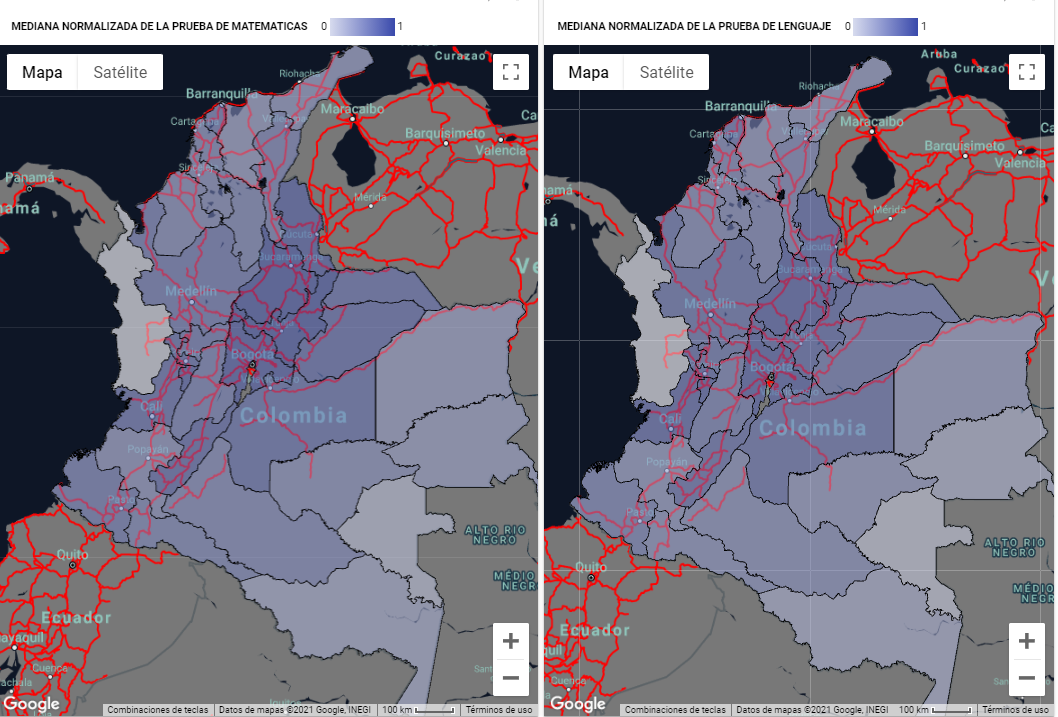
\includegraphics[scale=0.3]{Adjuntos/Roads_score.png} 
    \caption{\justifying{\small{ The spatial relationship between tests Saber11 road coverage at a departmental scale. The red line indicates the road network, and the polygons in the gray-to-blue scale show the scale of results in the saber 11 test.}}} 
    \label{fig:Figintro}
\end{figure}
\begin{center}
       \textbf{ Is this correlation hidding a causal effect of the roads infraestructure over the education performance?} 
    \end{center}
\end{frame}


% % ----------------- %new frame ---------------------------- % % 

\begin{frame}{Here's what I did.}
\justifying

    \begin{block}{Research question:}
     Does the intervention of roads under a concession contract have an impact on education in Colombia?
    \end{block}
 
    
 \end{frame}
 
% % ----------------- %new frame ---------------------------- % %

\begin{frame}{Contribution \hyperlink{rev.literature}{\beamerbutton{Literature Review}} }
     \label{contribution}
     
This study contribute to the literature showing \textbf{evidence that road concession agreements in Colombia impacts education} in the following outcomes:

\begin{itemize}
        \item Heterogeneous effects on private and public schools.
        \item Effect on labor force participation of students in the last year of secondary.
        \item Effect on human capital accumulation.
        \item Estimation of causality when the treatment occurs in continuous time.
  \end{itemize}
     %boton que me lleve a la literatura
\end{frame}

%%--------------------------------------------------------

\begin{frame}{Here's what I found.}
    \begin{itemize}
    \item   I find an increase in average reading and math scores in schools located less than a kilometer from the road intervention.
    % \pause
    \item In the early stages of  the road intervention, I find an increase in average reading and math scores mainly in schools located less than 1,500 meters from the road under construction.
    \item   In the final stages of the road intervention, I find an increase in average reading and math scores mainly in schools located more than 2,500 meters from the road.

    % \pause
    \item   The fraction of students who participate in the labor force decreases while the fraction of students completing some level of higher education increases, which leads to an accumulation of human capital.
    % \pause
    \item   The fraction of students from treated schools who complete a university degree increases. 
    % \pause
    \item   I show evidence of positive heterogeneous effects that affect public schools more than private schools.
 \end{itemize}
\end{frame}
%%--------------------------------------------------------
 
% % \hyperlink{context}{\beamerbutton{Back!}}  
 
% \end{frame}

%---------------------------DATA --------------------------- %
% \section{Data and Landscape.}

\begin{frame}{How?}{Data}
\label{data}

\justifying 

This study was carried through the following data:
\begin{itemize}
\justifying 
    \item General results and survey of the standardized exam of the last year of high school called Saber 11. (2006-2020) \hyperlink{education}{\beamerbutton{Education}}\label{contribution} % boton
    \item General results of the state test for the last semesters pot-secondary education students, called Saber pro (2006-2021).  % boton
    \item Vector of roads databases in Colombia. (2011-2019)
    \item Vector of schools databases in Colombia (DANE).  
    \item  Electronic survey of formal education – EDUC (C600).     
    \item  Road concession agreements and annual progress reports.
\end{itemize}

\end{frame}
% %--------------------New section---------------------------
%-------------------- Sección ---------------------------
\section{Empirical Srategy}

% % %--------------------New section---------------------------
 \section{Mechanisms}
 \begin{frame}{Mechanisms} \label{roads2} 
\begin{figure} [H]
    \centering
    \renewcommand\thefigure{3.1}
     \includegraphics[scale=0.5]{Graph/summarize mechanism.png}
    \caption{\justifying{Summary of the mechanism through which road construction under a concession agreement affects educational performance.}} 
    \label{fig:Figdispertion}
\end{figure}
\begin{center}
{Road Intervention}    $ \Rightarrow   \uparrow w_F     \Rightarrow   \downarrow L  	\Rightarrow    \uparrow s \Rightarrow \dot{H} $  \footnote{\tiny Where $w_F$ is the Income family,   $L$ is the labor force participation, $s$ is the studying time and $\dot{H}$ refers to human capital accumulation}
\end{center}
 \end{frame}

%-----------------------------New   Frame---------------------%
\begin{frame}{Treated and Control}
    \label{concession}
\begin{figure}[H]
    \centering
    \renewcommand\thefigure{4.2}
     \includegraphics[scale=0.25]{Graph/treat_control_schema.png}\\      
\end{figure}
    \footnotesize {Location of schools treated (green vignettes) and control schools (red vignettes) due to the construction of roads in the time of reference $t$.    }
\begin{figure}[H]
    \centering
    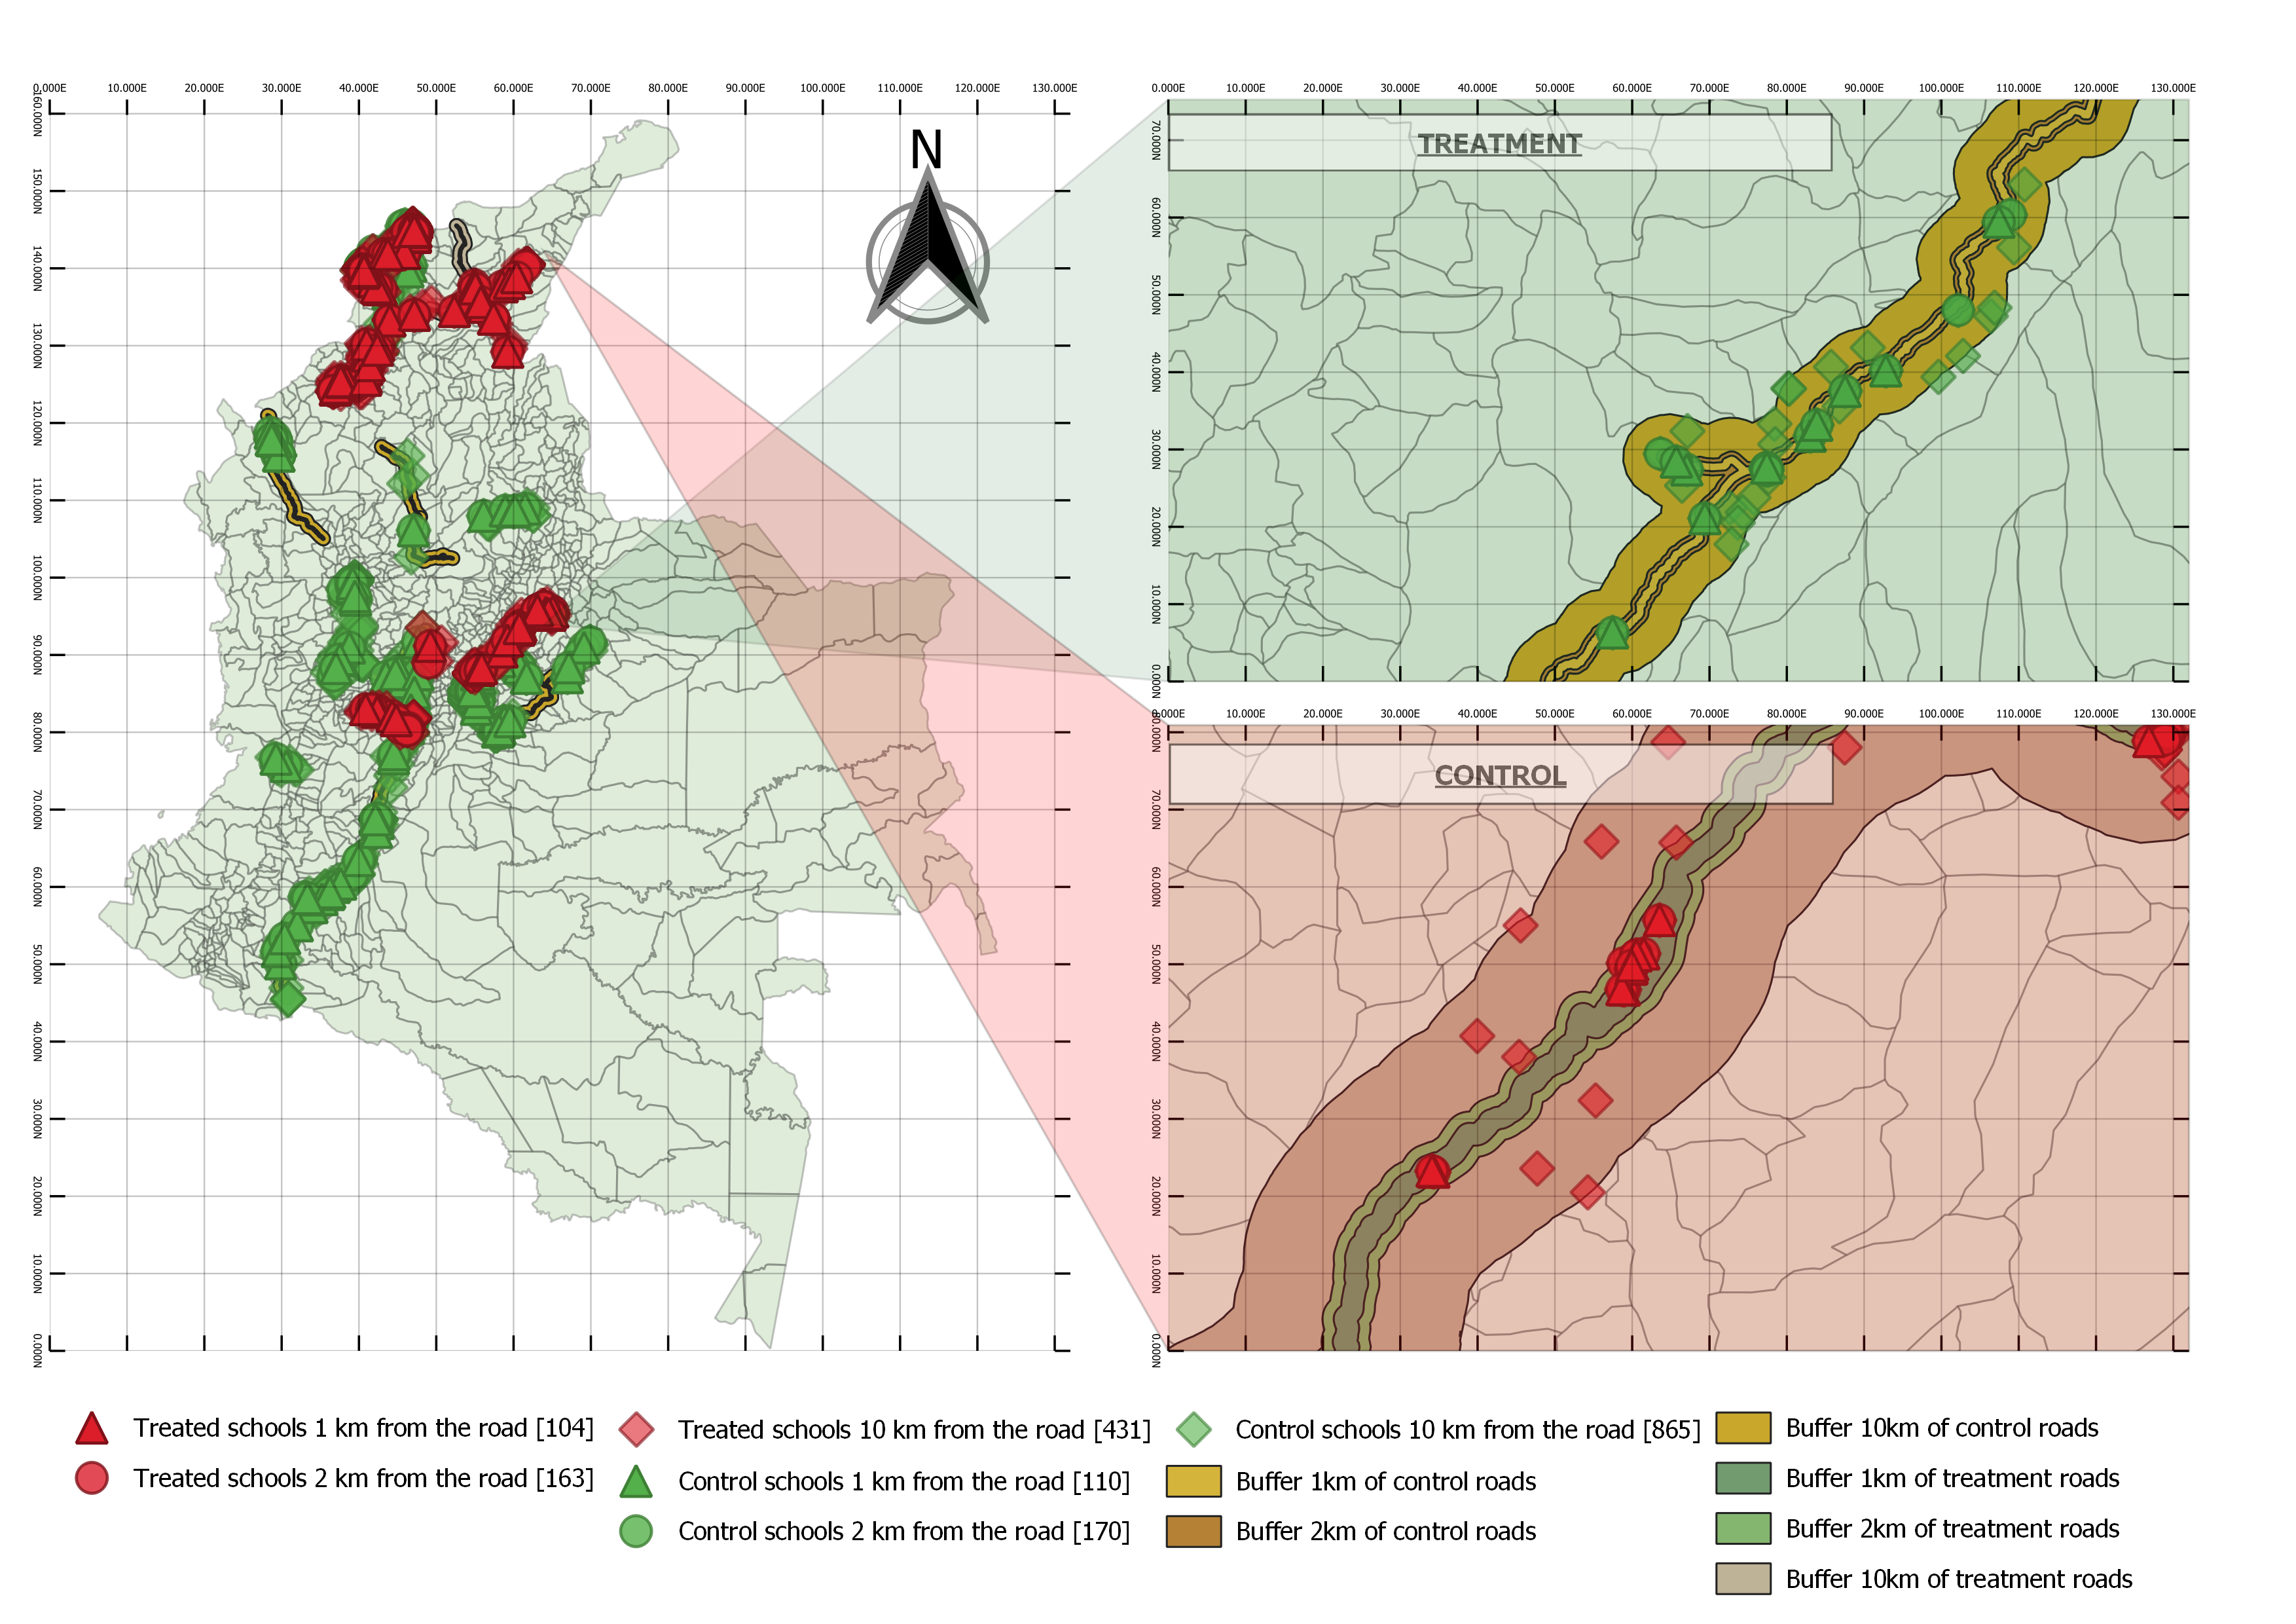
\includegraphics[scale=0.25]{Graph/Mapa de buffer4.png}  
\end{figure}

\end{frame}



%--------Method
\begin{frame}{Method}

\begin{itemize}
   
\item \textbf{Dynamic difference-in-difference model} stimation is based on:
    \begin{itemize}
        \item Two ways fixed effects estimators.
        \item the estimator proposed by    \cite{CALLAWAY2021200}, 
        \item the estimator proposed by   \cite{SUN2021175}
    \end{itemize}

\item \textbf{Assumptions  \cite{SUN2021175}}
      \begin{itemize}
            \item Parallel trends,
            \item No anticipatory behavior, 
            \item Treatment effect heterogeneity.  
    \end{itemize}

\item \textbf{ The two sources of variation are:}        
        
    \begin{itemize}
        \item Contruction of the road. (The time of contruction or whether the cosntruction was or not)
        
        \item  Distance between schools and roads contructed. 
    \end{itemize}

\end{itemize}

\end{frame}

%--------Specification
\begin{frame}{Specification}

\begin{equation} 
\hat{\tau} = \bar{Score}_{before road} - \bar{Score}_{after road}
\end{equation}

\begin{equation}  \label{eq:es1}
         Score_{c,t,j}^{\varphi} = %\beta_0 +
         \sum^{-2}_{\tau =-S}  \mu_\tau  \cdot D_{c,\tau} +
         \sum^{M}_{\tau =0}  \mu_\tau  \cdot D_{c,\tau} +
         \sigma_t +  + \gamma_c +  \varepsilon_{c,t} 
\end{equation} 

Where:
 \small
 
\begin{itemize}
    \item $t=-1$ Period relative to the treatment.\\
    \item  $ \gamma_c $ School fixed effects.\\
    \item $\sigma_t$ time fixed effects.\\
    \item$Score_{c,t,j} $ Is the outcome.\\
     %   The normalized standard-deviation  of the score obtained by the median behavior of the school $c$  in the subject $j$, in time $t$.
    \item$\mu_\varphi$ Is the effect of road construction on education.\\
    \item The effect of the construction of new roads is estimated with the bandwidth from $-S$ to $M$.\\
    \item $D_{c,\varphi}$ Represent a group of dummie variables that indicate the distance of each period from the treatment period.
 
\end{itemize}

\end{frame}
% % %----------------------------------------------------------
\begin{frame}{Estimation problem.}
        \begin{figure}[H]
    \centering
        \renewcommand\thefigure{4.2}
    \includegraphics[scale=0.46]{Graph/DID_‎Continuous_time.png}  
     
\end{figure}
\end{frame}
% % %----------------------------------------------------------
\begin{frame}{Estimation problem.}
        \begin{figure}[H]
    \centering
     
    \includegraphics[scale=0.35]{Graph/proposed_solution_time_continuos.png}  
     
\end{figure}
\end{frame}
% proposed_solution_time_continuos
% % %--------------------New section---------------------------
% \begin{frame}{Contexto} \label{roads2} 
% Características de vías en Colombia.  
% % \hyperlink{context}{\beamerbutton{Back!}}  
% \begin{center}
% \centering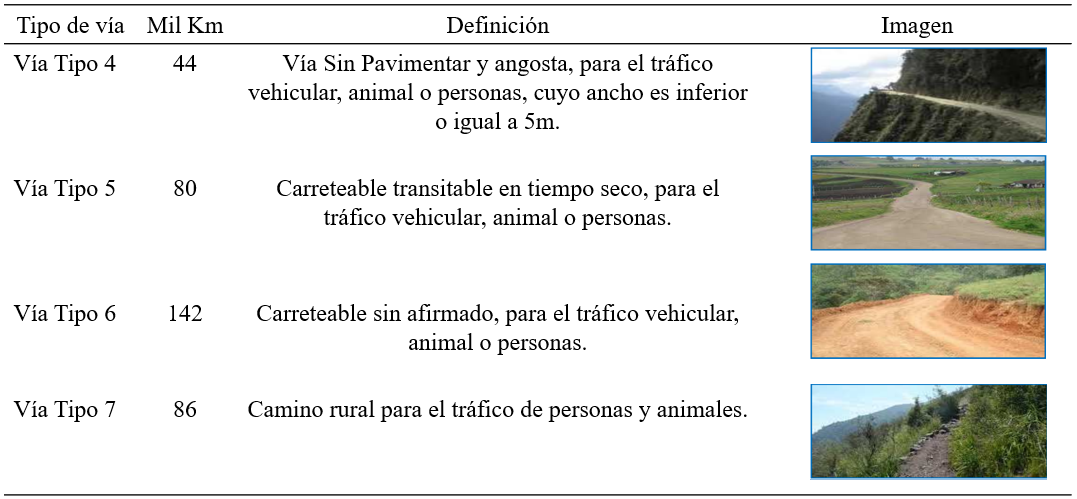
\includegraphics[scale=0.4]{Adjuntos/road2.png}
% \end{center}
% \caption{Base cartográfica IGAC}
% \end{frame}

 
% %--------------------New section---------------------------
\section{Results}
% %--------------------New frame---------------------------

\begin{frame}{Effect size of Results  } \label{size}

\begin{table}[]
% \caption{}
 
\begin{tabular}{llllllll}
\hline
\multicolumn{8}{c}{Effect size}                                                                                         \\ \hline
                  & \multicolumn{2}{c}{Overall} & \multicolumn{2}{c}{Math}  & \multicolumn{2}{c}{Reading} & Enrollment  \\ \hline
Effect size       & $sd^1$  & $sd^2$  & $sd^1$ & $sd^2$  & $sd^1$  & $sd^2$ & $sd^1$  \\
Small             & 0.08         & 0.04         & 0.05        & 0.08        & 0.03         & 0.08         & 0.03        \\
Moderate          & 0.1          & 0.1          & 0.07        & 0.07        & 0.14         & 0.12         & 0.06        \\
Large             & 0.45         & 0.47         & 0.31        & 0.37        & 0.5          & 0.5          & 0.38        \\
Number of studies & 96           & 747          & 199         & 314         & 269          & 495          & 33          \\ \hline
\end{tabular}
 
 \begin{tablenotes}
      \small
      \textbf{Note: } $sd^1$ refers to the studies carried out by Evanz, 2022 and 
      $sd^2$ refers to the studies carried out by Kraft, 2020.The distribution of sample size is based on all RCT studies  
       
    \end{tablenotes}
\end{table}
    
\end{frame}

%%%-------------------------------------------------------%%%
\subsection{Results in labor force participation}
%%%-------------------------------------------------------%%%

\begin{frame}{Human capital accumulation}
\small Impact of Roads on average results of exam Saber 11 in reading literacy score.  \hyperlink{A 3.5}{\beamerbutton{ Heterogenities by schools nature!}}   
\hyperlink{A 3.6}{\beamerbutton{Heterogenities by distance}}

\begin{equation}
    \dot{h}(t) = \phi(s(t),h(t)) - \delta_{h}h(t) 
\end{equation}
 Acemoglu 2010 \cite{acemoglu}- The Ben-Porath model

\begin{center} 
     \begin{figure}[H]
         \centering
         \includegraphics[scale = 0.25]{Graph/labor_force_10p.png}
         \caption{Impact on the fraction of students who participate in labor force }
         \label{fig:labor_force_10p}
     \end{figure}
\end{center}  
 %%%----------------------------------------------------------
%%%-------------------------------------------------------%%%
%%%-------------------------------------------------------%%%
% %--------------------New section---------------------------   
\end{frame}


%%%-------------------------------------------------------%%%

\begin{frame}{Fraction of students who participate in labor force} \label{result_labor}
     \begin{center} \label{tab:B.3} 
 \tiny
% \centering
\begin{tabular}{lccc}
   \tabularnewline \midrule \midrule
   Dependent Variable: & \multicolumn{3}{c}{Fraction of students who participate in labor force}\\
 Model by level of construction   :       & 10 \%    \hyperlink{10p_labor}{\beamerbutton{ graph!}}        & 50 \%    \hyperlink{50p_labor}{\beamerbutton{ graph!}}          & 100 \%    \hyperlink{100p_labor}{\beamerbutton{ graph!}}   \\    \midrule
   \emph{Variables}\\
   year $=$ -8  & 0.3341  (0.1894)    & 0.0429    (0.0866)        & 0.1899 (0.0966)\\   
                % &       &       & \\   
   year $=$ -7  & 0.1566   (0.3387)         & 0.3807 (0.0985) & -0.0574  (0.0787)\\   
                % &       &         &\\   
   year $=$ -6  & 0.0765 (0.1561)            & 0.0685  (0.0815)          & 0.0028 (0.0843)\\   
                % &       &       & \\   
   year $=$ -5  & -0.0458   (0.1150)        & 0.0578    (0.0788)       & 0.1307 (0.0986)\\   
                % &       &        & \\   
   year $=$ -4  & 0.0415 (0.0910)           & 0.0709  (0.0756)        & 0.0286 (0.0820)\\   
                % &       &         & \\   
   year $=$ -3  & 0.2354 (0.0819)   & 0.0228   (0.0653)        & 0.0773 (0.0846)\\   
                % &       &        & \\   
   year $=$ -2  & 0.0879     (0.0945)        & -0.0199 (0.0528)           & 0.0933 (0.0941)\\   
                % &      &      & \\   
   year $=$ 0   & -0.0100  (0.0670)        & 0.0872 (0.0661)            & -0.0015 (0.0812)\\   
                % &        &       & \\   
   year $=$ 1   & -0.0506(0.0687)          & 0.0482(0.0779)          & -0.1120(0.0829)\\   
                % &        &        & \\   
   year $=$ 2   & -0.0279(0.0790)           & -0.1970(0.0759) & -0.0700(0.1469)\\   
                % &       &         & \\   
   year $=$ 3   & -0.0699(0.0825)           & -0.2323(0.0784) & 0.0070(0.1439)\\   
                % &       &         & \\   
   year $=$ 4   & 0.0377 (0.0947)           & 0.0151 (0.1105)          &   \\   
                % &        &         &   \\   
   year $=$ 5   & -0.0143 (0.0922)        & 0.1681 (0.2386)           &   \\   
                % &         &        &   \\   
   year $=$ 6   & -0.3295(0.0876)   & -0.3180(0.2464)         &   \\   
                % &       &         &   \\   
   year $=$ 7   & -0.2900(0.0868) & 0.1621(0.2181)           &   \\   
                % &         &        &   \\   
   year $=$ 8   & -0.2143(0.1088)   &                 &   \\   
                % &        &                 &   \\   
 
   \midrule
   \emph{Fixed-effects}\\
   id\_name     & Yes             & Yes             & Yes\\  
   year         & Yes             & Yes             & Yes\\  
   \midrule
   \emph{Fit statistics}\\
   Observations & 5,882           & 5,882           & 5,843\\  
   R$^2$        & 0.47454         & 0.47006         & 0.46806\\  
%   Within R$^2$ & 0.03010         & 0.02145         & 0.00789\\  
   \midrule
   \emph{Results by buffer}\\
   Buffer 1000 m - 3500 m  &  Graph\hyperlink{10p_labor_buf}{\beamerbutton{ !}}            &  Graph\hyperlink{50p_labor_buf}{\beamerbutton{ !}}             &  Graph\hyperlink{100p_labor_buf}{\beamerbutton{ !}}   \\  
    Nature of school &  Graph\hyperlink{10p_labor_nat}{\beamerbutton{ !}}            &  Graph\hyperlink{50p_labor_nat}{\beamerbutton{ !}}             &    \\   
   \midrule  
   \multicolumn{4}{l}{\emph{Clustered (id\_name) standard-errors in parentheses}}\\
  % \multicolumn{4}{l}{\emph{Signif. Codes: : 0.01, : 0.05, : 0.1}}\\
   \midrule
\end{tabular}
  \end{center}
\end{frame}
   

 
 

%%%-------------------------------------------------------%%%

%----------------------------------------------------------
\subsection{Results in mathematics}
% %--------------------New frame---------------------------

%%%%%%%%%%%%%%%%%%%%%%%%%%%%%%%%%%%%%%
%%%%%%%%%%%%% 100 p %%%%%%%%%%%%%%%%%%%%
\begin{frame}{Mathematics score for all the different stages of construction} 
\label{math100p}
Effect of road intervention at less than 2500 meters.
    \begin{figure}
      \centering
      % include first image
      \includegraphics[width=0.8\linewidth]{Graph/SA_math_score_by_nature_ent.png} 
      \caption{\small 100 \% advance of construction  }
      \label{fig:6.1sub-first}
    \end{figure}
\end{frame}

%%%%%%%%%%%%% 50 p %%%%%%%%%%%%%%%%%%%%
\begin{frame}{Mathematics score for all the different stages of construction}
    \begin{figure}
      \centering
      % include first image
      \includegraphics[width=0.8\linewidth]{Graph/SA_math_score_by_nature_50p.png} 
      \caption{\small 50 \% advance of construction  }
      \label{fig:6.1sub-first}
    \end{figure}
\end{frame}

%%%%%%%%%%%%% 10 p %%%%%%%%%%%%%%%%%%%%
\begin{frame}{Mathematics score for all the different stages of construction}
    \begin{figure}
      \centering
      % include first image
      \includegraphics[width=0.8\linewidth]{Graph/SA_math_score_by_nature_10p.png} 
      \caption{\small 10 \% advance of construction 
       \hyperlink{result_math}{\beamerbutton{ all results!} } }
      \label{fig:6.1sub-first}
    \end{figure}
\end{frame}
%%%%%%%%%%%%%%%%%%%%%%%%%%%%%%%%

%%%-------------------------------------------------------%%%
%%%-------------------------------------------------------%%%
%%%-------------------------------------------------------%%%

\subsection{Results in reading literacy}

%%%%%%%%%%%%% 100 p %%%%%%%%%%%%%%%%%%%%
\begin{frame}{Reading Literacy score for all the different stages of construction} 
\label{math100p}

    \begin{figure}
      \centering
      % include first image
      \includegraphics[width=0.8\linewidth]{Graph/SA_reading_score_by_nature_ent.png} 
      \caption{\small 100 \% advance of construction   }
      \label{fig:6.1sub-first}
    \end{figure}
\end{frame}

%%%%%%%%%%%%% 50 p %%%%%%%%%%%%%%%%%%%%
\begin{frame}{Reading Literacy score for all the different stages of construction}
    \begin{figure}
      \centering
      % include first image
      \includegraphics[width=0.8\linewidth]{Graph/SA_reading_score_by_nature_50p.png} 
      \caption{\small 50 \% advance of construction  }
      \label{fig:6.1sub-first}
    \end{figure}
\end{frame}

%%%%%%%%%%%%% 10 p %%%%%%%%%%%%%%%%%%%%
\begin{frame}{Reading Literacy score for all the different stages of construction}
    \begin{figure}
      \centering
      % include first image
      \includegraphics[width=0.8\linewidth]{Graph/SA_reading_score_by_nature_10p.png} 
      \caption{\small 10 \% advance of construction 
       \hyperlink{result_read_}{\beamerbutton{ all results!} } }
      \label{fig:6.1sub-first}
    \end{figure}
\end{frame}



%###############################################




%------------------------------------------------%
%------------------------------------------------%

%%%-------------------------------------------------------%%%
%%%-------------------------------------------------------%%%
% %--------------------New section---------------------------


%%%-------------------------------------------------------%%%
%%%-------------------------------------------------------%%%

\subsection{Results in university participation}
\begin{frame}{Results in university participation}
     
 \begin{center} \label{tab:B.4} 
 
Fraction of students that finished some university level for all the different stages of construction

 \tiny
     \begin{tabular}{lcc}
   \tabularnewline \midrule \midrule
   Dependent Variable: & \multicolumn{2}{c}{Fraction of students that finished some university level}\\
    Model by level of construction   :       & 10 \% advance          & 50 \% advance \\  
   \midrule
   \emph{Variables}\\
   year $=$ -3  & 0.0016         & -0.1275\\   
                & (0.0499)       & (0.1112)\\   
   year $=$ -2  & 0.0525         & 0.0038\\   
                & (0.0521)       & (0.1437)\\   
   year $=$ 0   & 0.0946   & -0.2892\\   
                & (0.0523)       & (0.1876)\\   
   year $=$ 1   & 0.1415 & 0.1260\\   
                & (0.0534)       & (0.1359)\\   
   year $=$ 2   & 0.1342  &   \\   
                & (0.0633)       &   \\   
   \midrule
   \emph{Fixed-effects}\\
   id\_name     & Yes            & Yes\\  
   year         & Yes            & Yes\\  
   \midrule
   \emph{Fit statistics}\\
   Observations & 3,101          & 3,101\\  
   R$^2$        & 0.67737        & 0.66500\\  
   Within R$^2$ & 0.00350        & 0.00206\\  
   \midrule \midrule
   \multicolumn{3}{l}{\emph{Clustered (id\_name) standard-errors in parentheses}}\\
  % \multicolumn{3}{l}{\emph{Signif. Codes: ***: 0.01, **: 0.05, *: 0.1}}\\
   \midrule
\end{tabular}
 \end{center}
 
\end{frame}




%%%-------------------------------------------------------%%%
%%%-------------------------------------------------------%%%
%%%-------------------------------------------------------%%%

% \begin{frame}{Results in math test } \label{result_math}
% \small Impact of Roads on average results of exam Saber 11 in mathematics 
% \hyperlink{math_pub_priv}{\beamerbutton{See heterogenities!}}   
% \hyperlink{math_dista}{\beamerbutton{See Robustness check!}}   
 

%   \begin{figure}[H]
%          \centering
          
%           \renewcommand\thefigure{5.1}
%          \includegraphics[scale = 0.3]{Graph/Math_10p_1000m.png}
%          \caption{\small Impact of Roads on average results of exam in mathematics of the last year of secondary education. The treatment time is the year in which the construction of the road has reached a ten percent advance the construction.}
%          \label{fig:Figura_1}
%      \end{figure}
  
    
% \end{frame}


% % %--------------------New section---------------------------
% \begin{frame}{ Results in reading literacy test.}\label{Result_read}
% \small Impact of Roads on average results of exam Saber 11 in reading literacy score. \hyperlink{A 3.3}{\beamerbutton{ Heterogenities by schools nature!}}   
% \hyperlink{A 3.4}{\beamerbutton{Heterogenities by distance}}

%       \begin{figure}[H]
%          \centering
%               \renewcommand\thefigure{5.2}
%          \includegraphics[scale = 0.3]{Graph/Reading_10p_1000m.png}
%          \caption{\small Impact of Roads on average results of exam in reading literacy of the last year of secondary education. The treatment time is the year in which the construction of the road has reached a ten percent advance the construction.}
%          \label{fig:Math_result_1k}
%      \end{figure}
    
% \end{frame}

% % %--------------------New section---------------------------
% \begin{frame}{Impact of Roads on human capital accumulation}
%  \begin{center} 
%      \begin{figure}[H]
%          \centering
%          \includegraphics[scale = 0.3]{Graph/SA_natu_Participate_saberpro_base_ic.png}
%          \caption{Impact on the fraction of students who finished a university study}
%          \label{fig:higher_school_ic}
%      \end{figure}
% \end{center} 
% \end{frame}

% %-------------------- Sección ---------------------------
\section{Conclusion}


%------conclusion
\begin{frame}{Conclusions}
\begin{itemize}
     \item I evidenced an increase in the score of the results of mathematics and language on the standardized test for schools near roads under a concession agreement.
    
    \item I evidenced that the effect of the construction of a road under a concession agreement on education mainly benefits schools less than one kilometer away. The effect on education disappears in schools that are more than 1.5 km away from the highway.

    \item The effect of building a road under a concession agreement is greater in private schools than in public schools.

    \item The labor force participation of students in colleges less than a kilometer away from the road under a concession agreement decreases.
    
    \item The fraction of students from treated schools who complete a university degree increases. 
    
    \item The educational cycle from high school to university is benefited by the construction of roads, which in this article I approach as the accumulation of human capital.
    
\end{itemize}

\end{frame}

%------discossion
\section{Discussion}
 
\begin{frame}
\centering
Road to the Future: Identifying Impacts of Roads
on Education in Colombia\\~\\

        Jaime Polanco-Jimenez \\
        
        \small  School of Economics and Management Sciences\\
        Pontifical Xavierian University\\~\\
        
        \footnotesize      \url{https://github.com/JAPJ182/ROAD_TO_THE_FUTURE}\\
        \url{https://sites.google.com/view/jaime-polanco/inicio} \\~\\
        
    
\includegraphics[scale=0.2]{Adjuntos/logo.jpg}
\end{frame}

% %--------------------New section---------------------------
\appendix %\section{Anexos}
% %--------------------New frame---------------------------
\begin{frame}{Characteristic of roads under a concession.}
\hyperlink{concession}{\beamerbutton{Back!}}   \label{concession_anexo}
\justifying 

\begin{itemize}
    \item The time periods required for a road construction under a concession is in average \textbf{13 years}.\\
    \item In average the time require for reaching the \textbf{10\%} advance is 7.25 years and 2 years more for reaching the \textbf{50\%} of advance of the road.
    \item he concession length had an average of \textbf{191 km}
    \begin{itemize}
        \item The shortest concession length was \textbf{31km}.
        \item he largest concession length was \textbf{491 km}.
    \end{itemize}
    \item 987  schools (Public 737, Private 250 ) were implicated within a radius of 1000 meters from the road which represent the focus of this research. 
    % \begin{itemize}
    %     \item[Public] 737 
    %     \item[Private] 250
    % \end{itemize}
\end{itemize}
             
             
%\end{center}

  \begin{figure} [h!]
    \centering
    \renewcommand\thefigure{4.1}
     \includegraphics[scale=0.25]{Graph/disipation of the effet.png}
    \caption{\justifying{The spatial dispersion of the effect of road construction on education.}} 
    \label{fig:Figdispertion}
\end{figure}


\end{frame}

% %--------------------New section---------------------------

\begin{frame}{Road concession system } \label{roads1} 
Road concession system \\~\\
\hyperlink{concession}{\beamerbutton{Back!}}   \label{concession_anexo}
% \hyperlink{context}{\beamerbutton{Back!}}  
 
\centering\includegraphics[scale=0.35]{Graph/road_bulding.png}
 
 
\end{frame}


 % %--------------------New section---------------------------
% %%%%%%%%%%%%% Ejemplo de heterogeneidades y robustes 
% \begin{frame}{Heterogeneities in math literacy score of students by nature of the school
% \hyperlink{result_math}{\beamerbutton{Back!}}  
% } \label{math_pub_priv}
%       \begin{figure}[h!]
 
%          \centering
%          \includegraphics[scale = 0.3]{Graph/SA_math_score_by_nature_10p.png}
%      \end{figure}

% \end{frame}

 % %--------------------New section---------------------------

% \begin{frame}{Impact of road construction on math score by distance of school from road
% \hyperlink{result_math}{\beamerbutton{Back!}}  
% } \label{math_dista}
% %\begin{center} 
%      \begin{figure}[h!]
   
%          \centering
%           \includegraphics[scale = 0.3]{Graph/SA_Math_base_10p_buffers.png}

%      \end{figure}
% \end{frame} 


% \begin{frame}{Heterogeneities in reading literacy score of students    by nature of the school
% \hyperlink{Result_read}{\beamerbutton{Back!}} }
%     \label{A 3.3}
% \begin{figure}[H]
%  \renewcommand\thefigure{A 3.3}
%      \centering
%      \includegraphics[scale = 0.3]{Graph/SA_reading_score_by_nature_10p.png}
%       \caption{Heterogeneities in reading literacy score of students    by nature of the school 
%          \hyperlink{Reading_results}{.}}
%      \end{figure}

% \end{frame}


% \begin{frame}{Impact of road construction on reading literacy score by distance of school from road
% \hyperlink{Result_read}{\beamerbutton{Back!}} }
%      \label{A 3.4}
% \begin{figure}[H]
%  \renewcommand\thefigure{A 3.4}
%      \centering
%      \includegraphics[scale = 0.3]{Graph/SA_Reading_base_10p_buffers.png}
%      \caption{ \hyperlink{Reading_results}{.}}
%      \end{figure}

% \end{frame}
%--------------------------------------------------------

%--------------------------------------------------------

% \begin{frame}{Heterogeneities in Fraction of students from schools who just to work  by nature of the school
% \hyperlink{fig:Math_result_1k}{\beamerbutton{Back!}} }
%      \label{A 3.5}
% \begin{figure}[h!]
%  \renewcommand\thefigure{A 3.5}
%      \centering
%      \includegraphics[scale = 0.3]{Graph/SA_natu_labor_force_base10p.png}
%     \label{fig:Figura_7}
%   \end{figure}

% \end{frame}

% \begin{frame}{Impact of road construction on school share of labor force participation by distance of school from road
% \hyperlink{fig:Math_result_1k}{\beamerbutton{Back!}} }
%      \label{A 3.6}
% \begin{figure}[h!]
%  \renewcommand\thefigure{A 3.6}
%      \centering
%      \includegraphics[scale = 0.3]{Graph/SA_labor_force_10p_ALL_BUFFER.png}
     
%   \label{fig:Figura_7}
%   \end{figure}

% \end{frame}
%%%

%--------this paper
\begin{frame}{This paper. \hyperlink{contribution}{\beamerbutton{Back!}}}
\label{rev.literature}
\justifying 
What do we already know?
    \begin{itemize}
      
            \item   \cite{Adukia2020} Children \textbf{stay in school longer and perform better on standardized tests} as an effect of 115,000 new roads.
            \item    \cite{Donaldson2010} Railroads infrastructure  \textbf{decreased trade costs} and \textbf{interregional price gaps}, \textbf{increased interregional} and \textbf{international trade} and \textbf{increased real income levels}.
            \item  \cite{Fernandez2020} shows how transportation infrastructure \textbf{promoted long-term employment opportunities} and \textbf{broke the labor bond between parents and children}.
            \item   \cite{Fernald1999} Changes in roads has an \textbf{effect over the productivity} are mainly reflected in the intensive automotive production.
            \item   \cite{Sinisterra} (\textbf{Colombia 1993-2012})  Measures road improvement and construction as a function of production and inequality.
       
    \end{itemize}

    
\end{frame}

%---------------------------DATA --------------------------- %
\begin{frame}{ Education in colombia. \hyperlink{data}{\beamerbutton{Back!}}} \label{education}

\justifying 
    %\begin{center}
\begin{itemize}

    \item 1780 secondary schools were located with API and made up the sample.
    \item \textbf{987 schools} were implicated within a radius of 1000 meters from the road.
    \begin{itemize}
            \item 250 Private schools and 737 Public.
    \end{itemize}
    \item \textbf{12.9\%} and \textbf{10.4\%} were  \textbf{the percentage of students who partisipated in labor force} in private and public schools, respectively.
        
    \item \textbf{Public Schools} can not select their teachers due to the fact that teachers obtain their positions through merit contests.
     \item \textbf{Private Schools} can select their teachers and teachers can select the school where they want to work.
    \begin{itemize}
        \item By seeing improvements in the infrastructure a teacher with better qualities could select a school and this could impact in the school achievements.
    \end{itemize}
\end{itemize}
   \end{frame}     
   
                %-------------------------------%   
%-------------------------------%
                %-------------------------------%

\begin{frame}{A frame of reference for the impacts on education.}
\hyperlink{data}{\beamerbutton{Back!}}
\begin{center}
\begin{table}[h!]
\caption{Descriptive statistics of schools within a radius of 1000 meters from the road}
\label{tab:my-table}
\begin{tabular}{lllll}
\hline
\multicolumn{5}{c}{Schools within a radius of 1000 meters from the road} \\ \hline
& \multicolumn{2}{c}{Treated schools} & \multicolumn{2}{c}{Control Schools} \\ \cline{2-5} 
& mean & sd & mean & sd \\ \hline
Students with university studies * & 0.148 & 0.192 & 0.127 & 0.165 \\
Students in labor force + & 0.101 & 0.162 & 0.142 & 0.197 \\
Reading literacy Score & 0.491 & 0.057 & 0.484 & 0.051 \\
Mathematics score & 0.433 & 0.082 & 0.425 & 0.074 \\ \hline
Number of schools & \multicolumn{2}{c}{510} & \multicolumn{2}{c}{485} \\
Number of observations & \multicolumn{2}{c}{6565} & \multicolumn{2}{c}{5981} \\ \hline
\end{tabular}
\end{table}
\begin{threeparttable}
\begin{tablenotes}
\small
\item[*] Fraction of students who finished a university study,
\item[+] Fraction of students who participate in labor force
\end{tablenotes}
\end{threeparttable}
\end{center}  
\end{frame}

%\begin{frame}{Fraction of students who have completed any grade of university
%\hyperlink{fig:Math_result_1k}{\beamerbutton{Back!}} }
%     \label{A 3.8}
%\begin{figure}[h!]
% \renewcommand\thefigure{A 3.8}
%     \centering
%     \includegraphics[scale = 0.4]{Graph/SA_Participate_saberpro_base_ic_ALL_BUFFER_.png}
%     \caption{Fraction of students who have completed any grade of university
%         \hyperlink{fig:labor_force_10p}{.}}
         
%  \label{fig:Figura_8}
%   \end{figure}

%\end{frame}


% \end{center}
% %--------------------New section---------------------------
% %--------------------New section---------------------------
% %--------------------New section---------------------------
%%%------------------------------------------------------%%%
%%%------------------------------------------------------%%%
%%%%%%%%%%%%%%%%%%%%%%%%%%%%%%%%%%%%%%%%%%%%%%%%%%%%%%%%%%%%%%%%%%%%%%%%%%%%%%%%%%%%%%%%%%
%%%%%%%%%%%%%%%%%%%%%%%%%%%%%%%%%%%%%%%%%%%%%%%%%%%%%%%%%%%%%%%%%%%%%%%%%%%%%%%%%%%%%%%%%%

% %--------------------New frame---------------------------
\begin{frame}{Results in math test. \hyperlink{result_math}{\beamerbutton{Back!}}} \label{50p_math}
Impact of Roads on average results of exam Saber 11 in mathematics
\begin{figure}
  \centering
  % include first image
  \includegraphics[width=0.8\linewidth]{Graph/Math_50p_1000m.png} 
  \caption{\small 50 \% advance of construction}
  \label{fig:6.1sub-first}
\end{figure}
\end{frame}
% %--------------------New frame---------------------------
\begin{frame}{Results in math test. \hyperlink{result_math}{\beamerbutton{Back!}} } \label{100p_math}
Impact of Roads on average results of exam Saber 11 in mathematics
\begin{figure}
  \centering
  % include first image
  \includegraphics[width=0.8\linewidth]{Graph/Math_100p_1000m.png} 
  \caption{\small 100 \% advance of construction}
 
\end{figure}

\end{frame}

                            %%%%%%%%%%%%%%%%%%%%%%% 

                            %%%%%%%%%%%%%%%%%%%%%%% 



\begin{frame}{ Results in math test.  \hyperlink{result_math}{\beamerbutton{Back!}} }\label{10p_math_buf}
\small Impact of road construction on math score by distance of school from road in Math Result
\begin{figure}
  \centering
  % include first image
  \includegraphics[width=0.8\linewidth]{Graph/SA_Math_base_10p_buffers.png} 
  \caption{\small 10 \% advance of construction}
  \label{fig:6.1sub-first}
\end{figure}

\end{frame}
% %--------------------New frame---------------------------
\begin{frame}{ Results in math test.  \hyperlink{result_math}{\beamerbutton{Back!}} }\label{50p_math_buf}
\small Impact of road construction on math score by distance of school from road in Math Result
\begin{figure}
  \centering
  % include first image
  \includegraphics[width=0.8\linewidth]{Graph/SA_Math_base_50p_buffers.png} 
  \caption{\small 50 \% advance of construction}
  \label{fig:6.1sub-first}
\end{figure}

\end{frame}
% %--------------------New frame---------------------------
\begin{frame}{ Results in math test.   \hyperlink{result_math}{\beamerbutton{Back!}} }\label{100p_math_buf}
\small Impact of road construction on math score by distance of school from road in Math Result
\begin{figure}
  \centering
  % include first image
  \includegraphics[width=0.8\linewidth]{Graph/SA_Math_base_100p_buffers.png} 
  \caption{\small 100 \% advance of construction}
 
\end{figure}

\end{frame}



                            %%%%%%%%%%%%%%%%%%%%%%% 

                            %%%%%%%%%%%%%%%%%%%%%%% 


\begin{frame}{ Results in math test.  \hyperlink{result_math}{\beamerbutton{Back!}} }\label{10p_math_nat}
\small Estimation of heterogeneities (\cite{SUN2021175} estimator) in mathematics results according to the nature of the school  
\begin{figure}
  \centering
  \includegraphics[width=0.8\linewidth]{Graph/SA_reading_score_by_nature_10p.png} 
  \caption{\small 10 \% advance of construction}
  \label{fig:6.1sub-first}
\end{figure}
\end{frame}

\begin{frame}{ Results in math test.  \hyperlink{result_math}{\beamerbutton{Back!}} }\label{50p_math_nat}
\small Estimation of heterogeneities (\cite{SUN2021175} estimator) in mathematics results according to the nature of the school  
\begin{figure}
  \centering
  \includegraphics[width=0.8\linewidth]{Graph/SA_reading_score_by_nature_50p.png} 
  \caption{\small 50 \% advance of construction}
  \label{fig:6.1sub-first}
\end{figure}
\end{frame}

\begin{frame}{ Results in math test.  \hyperlink{result_math}{\beamerbutton{Back!}} }\label{100p_math_nat}
\small Estimation of heterogeneities (\cite{SUN2021175} estimator) in mathematics results according to the nature of the school  
\begin{figure}
  \centering
  \includegraphics[width=0.8\linewidth]{Graph/SA_reading_score_by_nature_ent.png} 
  \caption{\small 100 \% advance of construction}
  \label{fig:6.1sub-first}
\end{figure}
\end{frame}


%%%%%%%%%%%%%%%%%%%%%%%%%%%%%%%%%%%%%%%%%%%%%%%%%%%%%%%%%%%%%%%%%%%%%%%%%%%%%%%%%%%%%%%%%%
%%%%%%%%%%%%%%%%%%%%%%%%%%%%%%%%%%%%%%%%%%%%%%%%%%%%%%%%%%%%%%%%%%%%%%%%%%%%%%%%%%%%%%%%%%

%%%------------------------------------------------------%%%%
\begin{frame}{ Results in reading literacy test.  \hyperlink{result_read_}{\beamerbutton{Back!}} } \label{10p_read}
Impact of Roads on average results of exam Saber 11 in reading literacy score.
\begin{figure}
  \centering
  % include first image
  \includegraphics[width=0.8\linewidth]{Graph/Reading_10p_1000m.png} 
  \caption{\small 10 \% advance of construction}
  \label{fig:6.1sub-first}
\end{figure}

\end{frame}
% %--------------------New frame---------------------------
\begin{frame}{ Results in reading literacy test.  \hyperlink{result_read_}{\beamerbutton{Back!}}  }\label{50p_read}
Impact of Roads on average results of exam Saber 11 in reading literacy score.
\begin{figure}
  \centering
  % include first image
  \includegraphics[width=0.8\linewidth]{Graph/Reading_50p_1000m.png} 
  \caption{\small 50 \% advance of construction}
  \label{fig:6.1sub-first}
\end{figure}

\end{frame}
% %--------------------New frame---------------------------
\begin{frame}{ Results in reading literacy test.   \hyperlink{result_read_}{\beamerbutton{Back!}} }\label{100p_read}
Impact of Roads on average results of exam Saber 11 in reading literacy score.
\begin{figure}
  \centering
  % include first image
  \includegraphics[width=0.8\linewidth]{Graph/Reading_100p_1000m.png} 
  \caption{\small 100 \% advance of construction}
 
\end{figure}

\end{frame}



                            %%%%%%%%%%%%%%%%%%%%%%% 


\begin{frame}{ Results in reading literacy test.  \hyperlink{result_read_}{\beamerbutton{Back!}} }\label{10p_read_buf}
\small Impact of road construction on reading literacy score by distance of school from road 
\begin{figure}
  \centering
  % include first image
  \includegraphics[width=0.8\linewidth]{Graph/SA_Reading_base_10p_buffers.png} 
  \caption{\small 10 \% advance of construction}
  \label{fig:6.1sub-first}
\end{figure}

\end{frame}
% %--------------------New frame---------------------------
\begin{frame}{ Results in reading literacy test.  \hyperlink{result_read_}{\beamerbutton{Back!}} }\label{50p_read_buf}
\small Impact of road construction on reading literacy score by distance of school from road 
\begin{figure}
  \centering
  % include first image
  \includegraphics[width=0.8\linewidth]{Graph/SA_Reading_base_50p_buffers.png} 
  \caption{\small 50 \% advance of construction}
  \label{fig:6.1sub-first}
\end{figure}

\end{frame}
% %--------------------New frame---------------------------
\begin{frame}{ Results in reading literacy test.   \hyperlink{result_read_}{\beamerbutton{Back!}} }\label{100p_read_buf}
\small Impact of road construction on reading literacy score by distance of school from road 
\begin{figure}
  \centering
  % include first image
  \includegraphics[width=0.8\linewidth]{Graph/SA_Reading_base_100p_buffers.png} 
  \caption{\small 100 \% advance of construction}
 
\end{figure}

\end{frame}

                            %%%%%%%%%%%%%%%%%%%%%%%%%%%%%%%%%%%%%%%
                            %%%%%%%%%%%%%%%%%%%%%%%%%%%%%%%%%%%%%%%


\begin{frame}{ Results in reading literacy test.  \hyperlink{result_read_}{\beamerbutton{Back!}} }\label{10p_read_nat}
\small Heterogeneities in reading literacy score of students by nature of the schoo
\begin{figure}
  \centering
  \includegraphics[width=0.8\linewidth]{Graph/SA_reading_score_by_nature_10p.png} 
  \caption{\small 10 \% advance of construction}
  \label{fig:6.1sub-first}
\end{figure}

\end{frame}

\begin{frame}{ Results in reading literacy test.  \hyperlink{result_read_}{\beamerbutton{Back!}} }\label{50p_read_nat}
\small Heterogeneities in reading literacy score of students by nature of the schoo
\begin{figure}
  \centering
  \includegraphics[width=0.8\linewidth]{Graph/SA_reading_score_by_nature_50p.png} 
  \caption{\small 50 \% advance of construction}
  \label{fig:6.1sub-first}
\end{figure}

\end{frame}

\begin{frame}{ Results in reading literacy test.  \hyperlink{result_read_}{\beamerbutton{Back!}} }\label{100p_read_nat}
\small Heterogeneities in reading literacy score of students by nature of the schoo
\begin{figure}
  \centering
  \includegraphics[width=0.8\linewidth]{Graph/SA_reading_score_by_nature_ent.png} 
  \caption{\small 100 \% advance of construction}
  \label{fig:6.1sub-first}
\end{figure}

\end{frame}


%%%%%%%%%%%%%%%%%%%%%%%%%%%%%%%%%%%%%%%%%%%%%%%%%%%%%%%%%%%%%%%%%%%%%%%%%%%%%%%%%%%%%%%%%%
%%%%%%%%%%%%%%%%%%%%%%%%%%%%%%%%%%%%%%%%%%%%%%%%%%%%%%%%%%%%%%%%%%%%%%%%%%%%%%%%%%%%%%%%%%

\begin{frame}{ Results in labor force. \hyperlink{result_labor}{\beamerbutton{Back!}}  } \label{10p_labor}
Impact of Roads on average results on the fraction of students who participate in labor force in the last year of secondary education. 
\begin{figure}
  \centering
  % include first image
  \includegraphics[width=0.8\linewidth]{Graph/labor_force_10p_1000m.png} 
  \caption{\small 10 \% advance of construction}
  \label{fig:6.1sub-first}
\end{figure}

\end{frame}
 
\begin{frame}{ Results in labor force.\hyperlink{result_labor}{\beamerbutton{Back!}} }  \label{50p_labor}
Impact of Roads on average results on the fraction of students who participate in labor force in the last year of secondary education. 
\begin{figure}
  \centering
  % include first image
  \includegraphics[width=0.8\linewidth]{Graph/labor_force_50p_1000m.png} 
  \caption{\small 50 \% advance of construction}
  \label{fig:6.1sub-first}
\end{figure}

\end{frame}
% %--------------------New frame---------------------------

\begin{frame}{ Results in labor force.\hyperlink{result_labor}{\beamerbutton{Back!}} }\label{100p_labor}
Impact of Roads on average results on the fraction of students who participate in labor force in the last year of secondary education. 
\begin{figure}
  \centering
  % include first image
  \includegraphics[width=0.8\linewidth]{Graph/labor_force_100p_1000m.png} 
  \caption{\small 100 \% advance of construction}
 
\end{figure}

\end{frame}
 
                            %%%%%%%%%%%%%%%%%%%%%%%%%%%%%%%%%%%%%%%
                            %%%%%%%%%%%%%%%%%%%%%%%%%%%%%%%%%%%%%%%
                            
\begin{frame}{ Results in labor force. \hyperlink{result_labor}{\beamerbutton{Back!}}  } \label{10p_labor_buf}
Impact of Roads on average results on the fraction of students who participate in labor force in the last year of secondary education. 
\begin{figure}
  \centering
  % include first image
  \includegraphics[width=0.8\linewidth]{Graph/SA_estu_trabaja_base_10p_buffers.png} 
  \caption{\small 10 \% advance of construction}
  \label{fig:6.1sub-first}
\end{figure}

\end{frame}

% %--------------------New frame---------------------------
\begin{frame}{ Results in labor force.\hyperlink{result_labor}{\beamerbutton{Back!}} }  \label{50p_labor_buf}
Impact of Roads on average results on the fraction of students who participate in labor force in the last year of secondary education. 
\begin{figure}
  \centering
  % include first image
  \includegraphics[width=0.8\linewidth]{Graph/SA_estu_trabaja_base_50p_buffers.png} 
  \caption{\small 50 \% advance of construction}
  \label{fig:6.1sub-first}
\end{figure}

\end{frame}

% %--------------------New frame---------------------------
\begin{frame}{ Results in labor force.\hyperlink{result_labor}{\beamerbutton{Back!}} }\label{100p_labor_buf}
Impact of Roads on average results on the fraction of students who participate in labor force in the last year of secondary education. 
\begin{figure}
  \centering
  % include first image
  \includegraphics[width=0.8\linewidth]{Graph/SA_estu_trabaja_base_100p_buffers.png} 
  \caption{\small 100 \% advance of construction}
 
\end{figure}

\end{frame}

 
                            %%%%%%%%%%%%%%%%%%%%%%%%%%%%%%%%%%%%%%%
                            %%%%%%%%%%%%%%%%%%%%%%%%%%%%%%%%%%%%%%%

\begin{frame}{ Results in labor force. \hyperlink{result_labor}{\beamerbutton{Back!}}  } \label{10p_labor_nat}

Estimation of heterogeneities (Sun and Abraham, 2021 estimator) in labor force results according to the nature of the school.

\begin{figure}
  \centering
  % include first image
  \includegraphics[width=0.8\linewidth]{Graph/SA_labor_force_by_nature_10p.png} 
  \caption{\small 10 \% advance of construction}
  \label{fig:6.1sub-first}
\end{figure}

\end{frame}                            

\begin{frame}{ Results in labor force. \hyperlink{result_labor}{\beamerbutton{Back!}}  } \label{50p_labor_nat}

Estimation of heterogeneities (Sun and Abraham, 2021 estimator) in labor force results according to the nature of the school.

\begin{figure}
  \centering
  % include first image
  \includegraphics[width=0.8\linewidth]{Graph/SA_labor_force_by_nature_50p.png} 
  \caption{\small 50 \% advance of construction}
  \label{fig:6.1sub-first}
\end{figure}

\end{frame}   

 
%%-------------------------------------------------------
%-------------------- Sección ---------------------------
%%%%%%%%%%%%%%%%%%%%%%%%%%%%%%%

\begin{frame}{Mathematics score for all the different stages of construction 
\hyperlink{math100p}{\beamerbutton{Back!}}   } \label{result_math} 
    \begin{center} 
 
 \tiny
\centering
\begin{tabular}{lccc}
    % \tabularnewline \midrule \midrule
   Dependent Variable: & \multicolumn{3}{c}{score in mathematics}\\
   Model by level of construction   :       & 10 \%  \hyperlink{10p_math}{\beamerbutton{ graph!} }           & 50 \%  \hyperlink{50p_math}{\beamerbutton{ graph!} }          & 100 \%  \hyperlink{100p_math}{\beamerbutton{ graph!} }   \\  
   \midrule
   \emph{Variables}\\
   year $=$ -8  & -0.0149 (0.2195)          & 0.0173 (0.0804)         & -0.0844 (0.0676)\\   
   year $=$ -7  & 0.2077 (0.1964)           & 0.0208 (0.0699)          & -0.0026 (0.0734)\\   
   year $=$ -6  & -0.2923 (0.1077)   & -0.0347 (0.0587)       & 0.0872 (0.0760)\\   
   year $=$ -5  & -0.0940 (0.0818)         & 0.0280 (0.0583)          & -0.0266  (0.0747)\\   
   year $=$ -4  & -0.0654 (0.0796)        & 0.0510 (0.0532)         & 0.0550 (0.0624)\\    
   year $=$ -3  & -0.0328 (0.0691)          & 0.1018 (0.0494) & 0.0997 (0.0640)\\    
   year $=$ -2  & -0.0873  (0.0520)   & 0.1275 (0.0484) & 0.0562 (0.0658)\\    
   year $=$ 0   & 0.0039 (0.0518)          & 0.0319 (0.0455)         & 0.0926 (0.0616)\\    
   year $=$ 1   & 0.0830 (0.0549)         & 0.0869 (0.0494)  & 0.0878 (0.0619)\\    
   year $=$ 2   & 0.0967 (0.0568)     & 0.1465 (0.0537) & 0.1478 (0.0993)\\    
   year $=$ 3   & 0.0200 (0.0605)           & 0.1227 (0.0548)  & 0.1142 (0.0915)\\    
   year $=$ 4   & 0.0018  (0.0642)         & 0.0667 (0.0744)          &   \\    
   year $=$ 5   & 0.0695   (0.0607)        & -0.2395  (0.1893)       &   \\    
   year $=$ 6   & 0.0843 (0.0674)           & -0.2568   (0.1723)      &   \\    
   year $=$ 7   & 0.1164 (0.0671)    & -0.0735 (0.1711)        &   \\    
   year $=$ 8   & 0.2204  (0.0958)  &                &   \\    
 
   \midrule
   \emph{Fixed-effects}\\
   id\_name     & Yes             & Yes            & Yes\\  
   year         & Yes             & Yes            & Yes\\  
   \midrule
   \emph{Fit statistics}\\
   Observations & 5,882           & 5,882          & 5,843\\  
   R$^2$        & 0.73786         & 0.73699        & 0.73070\\  
%   Within R$^2$ & 0.01476         & 0.01370        & 0.00849\\  
   \midrule  
   \emph{Results by buffer}\\
   Buffer 1000 m - 3500 m  &  Graph\hyperlink{10p_math_buf}{\beamergotobutton{ }}            &  Graph\hyperlink{50p_math_buf}{\beamergotobutton{}}             &  Graph\hyperlink{100p_math_buf}{\beamergotobutton{}}     \\
    Nature of school &  .\hyperlink{10p_math_nat}{\beamerbutton{ !}}            &  .\hyperlink{50p_math_nat}{\beamerbutton{ !}}             &  .\hyperlink{100p_math_nat}{\beamerbutton{ !}}    \\   
   \midrule  
   \multicolumn{4}{l}{\emph{Clustered (id\_name) standard-errors in parentheses}}\\
   \multicolumn{4}{l}{\emph{Signif. Codes: : 0.01, : 0.05, : 0.1}}\\
   \midrule
\end{tabular}
 
 
 \end{center}
\end{frame}

%%%%%%%%%%%%%%%%%%%%%%%%%%%%%%5
%------------------------------------------------%
\begin{frame}{Reading literacy score for all stages of construction.  \hyperlink{math100p}{\beamerbutton{ back!} } 
} \label{result_read_}
    \begin{center}  
 
 \tiny
\centering
\begin{tabular}{lccc}
   \tabularnewline \midrule \midrule
   Dependent Variable: & \multicolumn{3}{c}{Reading literacy}\\
    Model by level of construction   :       & 10 \% \hyperlink{10p_read}{\beamerbutton{ graph!} }          & 50 \% \hyperlink{50p_read}{\beamerbutton{ graph!} }           & 100 \% \hyperlink{100p_read}{\beamerbutton{ graph!} }    \\  
   \midrule
   \emph{Variables}\\
   year $=$ -8  & -0.3852(0.1915) & -0.0521 (0.0651)         & -0.0552(0.0608)\\   
   year $=$ -7  & 0.2824(0.1017)   & -0.0701 (0.0594)        & -0.1408 (0.0635)\\
   year $=$ -6  & -0.0934  (0.0919)       & -0.0622 (0.0596)         & 0.0795 (0.0693)\\   
   year $=$ -5  & 0.0283 (0.0702)         & -0.0131 (0.0571)         & 0.0293 (0.0630)\\
   year $=$ -4  & -0.0446 (0.0714)        & 0.0176 (0.0523)         & 0.0857 (0.0590)\\
   year $=$ -3  & -0.0094 (0.0666)        & 0.1078 (0.0540)   & 0.0621 (0.0558)\\   
   year $=$ -2  & -0.0173  (0.0568)        & 0.0580 (0.0465)          & 0.1121 (0.0584)\\   
   year $=$ 0   & 0.0381 (0.0562)          & 0.0459 (0.0453)          & 0.1219 (0.0551)\\   
   year $=$ 1   & 0.1691 (0.0611)  & 0.1074 (0.0452)     & 0.0841 (0.0526)\\   
   year $=$ 2   & 0.1027 (0.0587)   & 0.1474 (0.0506)  & 0.0630 (0.0735)\\    
   year $=$ 3   & 0.0888 (0.0610)            & 0.1097 (0.0519)    & -0.0247 (0.0718)\\    
   year $=$ 4   & 0.0917 (0.0666)          & 0.0335 (0.0718)           &   \\   
   year $=$ 5   & 0.1497 (0.0615)  & -0.1309 (0.1534)        &   \\    
   year $=$ 6   & 0.1640 (0.0666)   & -0.1449 (0.1471)         &   \\
   year $=$ 7   & 0.1752 (0.0643)  & -0.0966 (0.1423)        &   \\   
   year $=$ 8   & 0.2455 (0.0982)   &                &   \\   
   \midrule
   \emph{Fixed-effects}\\
   id\_name     & Yes            & Yes            & Yes\\  
   year         & Yes            & Yes            & Yes\\  
   \midrule
   \emph{Fit statistics}\\
   Observations & 5,882          & 5,882          & 5,843\\  
   R$^2$        & 0.74701        & 0.74888        & 0.74911\\  
%   Within R$^2$ & 0.01748        & 0.01502        & 0.00854\\  
   \midrule  
   \emph{Results by buffer}\\
   Buffer 1000 m - 3500 m  &  .\hyperlink{10p_read_buf}{\beamergotobutton{ }}            &  .\hyperlink{50p_read_buf}{\beamergotobutton{}}             &  .\hyperlink{100p_read_buf}{\beamergotobutton{}}   \\  
    Nature of school &  .\hyperlink{10p_read_nat}{\beamerbutton{ }}            &  .\hyperlink{50p_read_nat}{\beamerbutton{ }}             &  .\hyperlink{100p_read_nat}{\beamerbutton{ }}    \\   
   \midrule  
   \multicolumn{4}{l}{\emph{Clustered (id\_name) standard-errors in parentheses}}\\
 %  \multicolumn{4}{l}{\emph{Signif. Codes: : 0.01, : 0.05, : 0.1}}\\
\midrule
\end{tabular}
%10p_read_nat
 
 \end{center}
\end{frame}


%%%----------------------------------------------------------

% %--------------------New frame---------------------------
\begin{frame}{What happened to the teachers?} \label{50p_math}
Public Schools.

\begin{figure}
  \centering
  \includegraphics[width=0.8\linewidth] {Graph/SA_profes_preg_by_nature_10p.png} 
  \caption{\small 10 \% advance of construction}
  \label{fig:6.1sub-first}
\end{figure}
\end{frame}
%% - --------------------

% %--------------------New frame---------------------------
\begin{frame}{Results in math test. \hyperlink{result_math}{\beamerbutton{Back!}}} \label{50p_math}
Impact of Roads on average results of exam Saber 11 in mathematics
\begin{figure}
  \centering
  % include first image
  \includegraphics[width=0.8\linewidth]{Graph/Math_50p_1000m.png} 
  \caption{\small 50 \% advance of construction}
  \label{fig:6.1sub-first}
\end{figure}
\end{frame}



\end{document}